%%%%%%%%%%%%%%%%%%%%%%%%%%%%%%%%%%%%%%%%%%%%%%%%%%%%%%%%%%%%%%%%%%%%%%%%%%%

\documentclass{standalone}

\usepackage{mathptmx}
\usepackage{tikz}
\usetikzlibrary{external}
\tikzexternalize{unit-circle}

%% We default to Times.
\renewcommand{\rmdefault}{ptm}
\renewcommand{\ttdefault}{pcr}
%% Enable Times/Palatino main text font.
\normalfont\selectfont

%% A unit circle.

\begin{document}

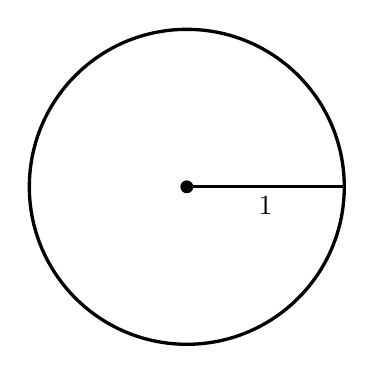
\begin{tikzpicture}[%%
  lineStyle/.style={-,very thick},%%
  originStyle/.style={draw,inner sep=1.5pt,circle,fill=black,black}
]
%%
%%
\pgfmathsetmacro{\radius}{2}
\pgfmathsetmacro{\xlow}{0}
\pgfmathsetmacro{\ylow}{0}
\coordinate (centre) at (\xlow,\ylow);
%%
%% Draw a unit circle.
%%
%% The circle and its centre.
\draw[lineStyle] (centre) circle[radius=\radius];
\node[originStyle] at (centre) {};
%% The radius of the circle.
\draw[lineStyle] (centre) -- (\radius,0);
\node at (\radius/2,\ylow) [below] {$1$};
\end{tikzpicture}

\end{document}
